\documentclass[11pt,a4paper,fontset=none]{ctexart}

\usepackage{fontspec}
\usepackage{xeCJK}
\usepackage[a4paper,top=2.2cm,bottom=2.1cm,left=2.15cm,right=2.15cm,headsep=0.8cm,footskip=0.9cm]{geometry}
\usepackage{xcolor}
\usepackage{graphicx}
\usepackage{hyperref}
\usepackage{fancyhdr}
\usepackage{caption}
\usepackage{float}
\usepackage{setspace}
\usepackage{titlesec}
\usepackage{booktabs}

\definecolor{ink}{HTML}{0C1C19}
\definecolor{sea}{HTML}{133F38}
\definecolor{seamist}{HTML}{799188}
\definecolor{ember}{HTML}{C95A3B}
\definecolor{mist}{HTML}{E8E2D7}
\definecolor{paper}{HTML}{FCFBF7}
\definecolor{stone}{HTML}{505E59}

\setmainfont{Noto Serif}
\setsansfont{Noto Sans}
\setmonofont{DejaVu Sans Mono}
\setCJKmainfont{Noto Serif CJK SC}
\setCJKsansfont{Noto Sans CJK SC}
\setCJKmonofont{Noto Sans Mono CJK SC}

\pagecolor{paper}
\color{ink}
\setlength{\parindent}{0pt}
\setlength{\parskip}{0.5em}
\onehalfspacing
\setlength{\headheight}{22pt}
\setcounter{secnumdepth}{0}

\hypersetup{
  colorlinks=true,
  linkcolor=sea,
  urlcolor=ember,
  citecolor=sea,
  pdftitle={DeepSeek的建模水平大幅提升},
  pdfauthor={朱华天，DeepSeek V4.1 Flash 1017},
  pdfsubject={Three.js 程序化建模：Cormorant C--7 与 SKYPRO XT},
  pdfkeywords={Three.js, USV, UAV, 程序化建模, DeepSeek, LaTeX}
}

\captionsetup{
  font={small,sf},
  labelfont={bf,color=ember},
  labelsep=period,
  textfont={color=stone},
  skip=6pt
}

\titleformat{\section}
  {\sffamily\LARGE\bfseries\color{sea}}
  {}{0em}{}
  [\vspace{-0.35em}{\color{mist}\rule{\linewidth}{0.5pt}}]
\titlespacing*{\section}{0pt}{0.7em}{0.7em}

\pagestyle{fancy}
\fancyhf{}
\renewcommand{\headrulewidth}{0.3pt}
\renewcommand{\headrule}{\hbox to\headwidth{\color{mist}\leaders\hrule height \headrulewidth\hfill}}
\fancyhead[L]{\sffamily\footnotesize\color{seamist}DEEPSEEK V4.1 FLASH 1017 / MODEL STUDY}
\fancyhead[R]{\sffamily\footnotesize\color{seamist}CORMORANT C–7 / SKYPRO XT}
\fancyfoot[L]{\sffamily\footnotesize\color{seamist}2026.10.18}
\fancyfoot[R]{\sffamily\footnotesize\color{seamist}\thepage}

\newcommand{\repo}{https://github.com/ZHT1235456/Three-js-USV-by-DeepSeek}
\newcommand{\repopath}{github.com/ZHT1235456/Three-js-USV-by-DeepSeek}
\newcommand{\eyebrow}[1]{{\sffamily\footnotesize\bfseries\color{ember}\MakeUppercase{#1}}}
\newcommand{\smallcapslabel}[1]{{\sffamily\footnotesize\color{seamist}#1}}

\begin{document}

\begin{titlepage}
\thispagestyle{empty}
\color{ink}
\vspace*{-0.35cm}
\noindent
{\sffamily\bfseries\small\color{sea}PELAGIC MARINE SYSTEMS}\hfill
{\sffamily\small\color{seamist}MODEL STUDY / 2026}

\vspace{0.25cm}
{\color{mist}\rule{\linewidth}{0.5pt}}

\vspace{1.5cm}
\noindent\eyebrow{THREE.JS · PROCEDURAL MODELING}\\[0.5cm]
{\fontsize{31}{38}\selectfont\bfseries
DeepSeek的建模水平\\[0.06em]
大幅提升\par}

\vspace{0.45cm}
{\color{ember}\rule{\linewidth}{1.7pt}}

\vspace{0.55cm}
{\Large\color{sea}海与空：Cormorant C–7 与 SKYPRO XT\\
程序化建模记录\par}

\vspace{0.9cm}
\begin{minipage}[t]{0.47\linewidth}
  {\smallcapslabel{作者}}\\[0.12cm]
  {\large 朱华天，DeepSeek V4.1 Flash 1017}
\end{minipage}\hfill
\begin{minipage}[t]{0.47\linewidth}
  {\smallcapslabel{日期}}\\[0.12cm]
  {\large 2026年10月18日}
\end{minipage}

\vspace{0.55cm}
\noindent
{\smallcapslabel{仓库}}\hspace{0.45cm}
{\small\href{\repo}{\texttt{\repopath}}}\par

\vfill
\begin{center}
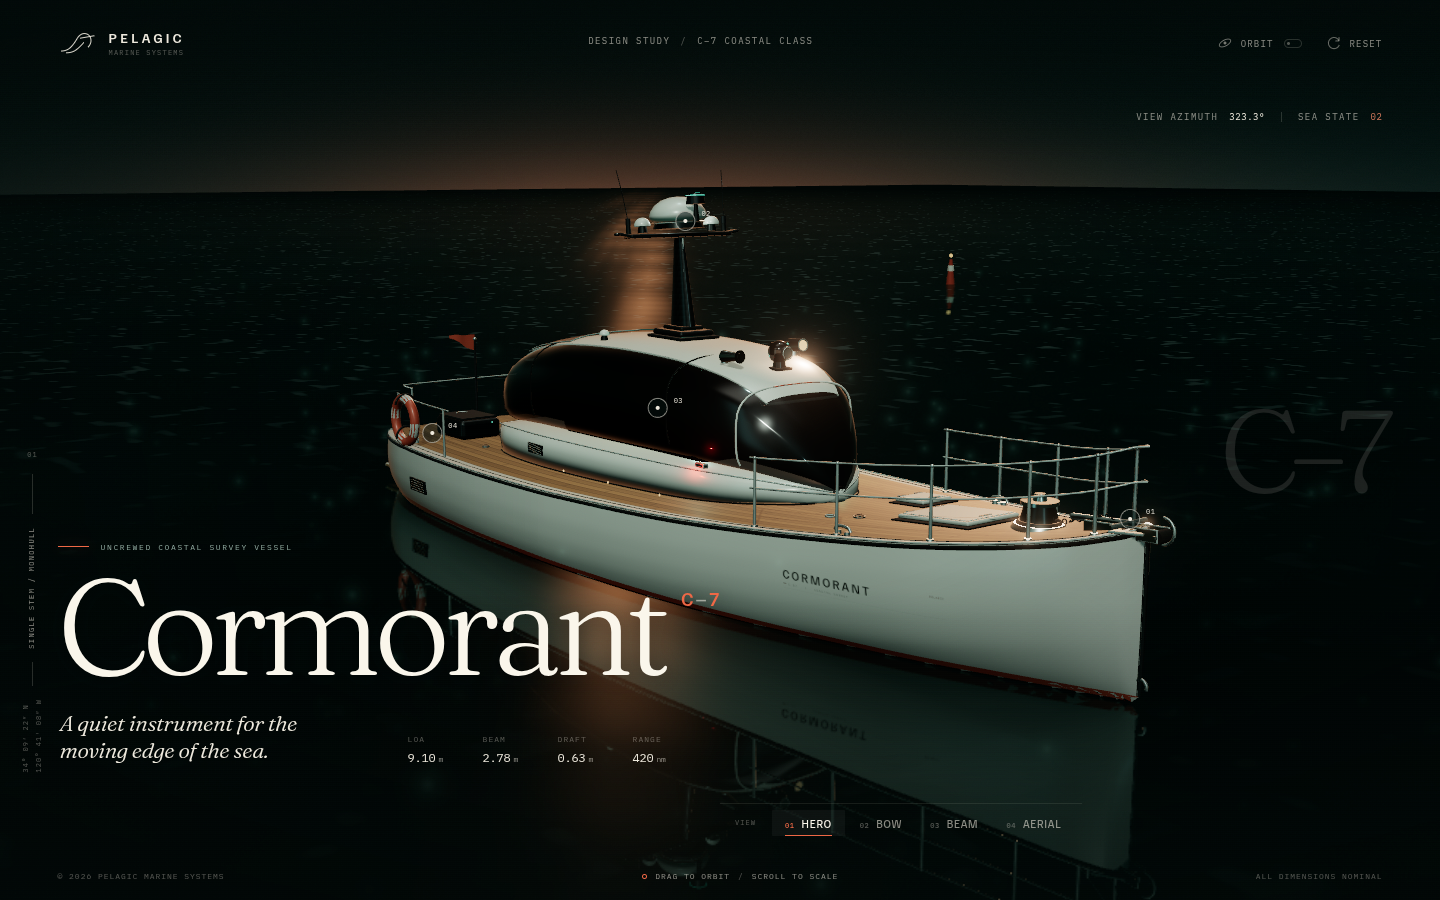
\includegraphics[width=\linewidth,height=8.0cm,keepaspectratio]{figures/hero.png}
\end{center}
\end{titlepage}

\section{海 / Cormorant C--7}

Cormorant C--7 是一艘 9.10\,m 单体尖艏无人测量艇。船体以 PCHIP 插值生成非均匀站位，放样为 $180\times32$ 的连续曲面；柚木甲板、烟色玻璃舱罩、传感器桅杆、锚链与双喷水推进器各自拥有独立的尺度与材质逻辑。全部几何、材质和纹理由 Three.js 与 Canvas 程序化生成。

\begin{figure}[H]
\centering
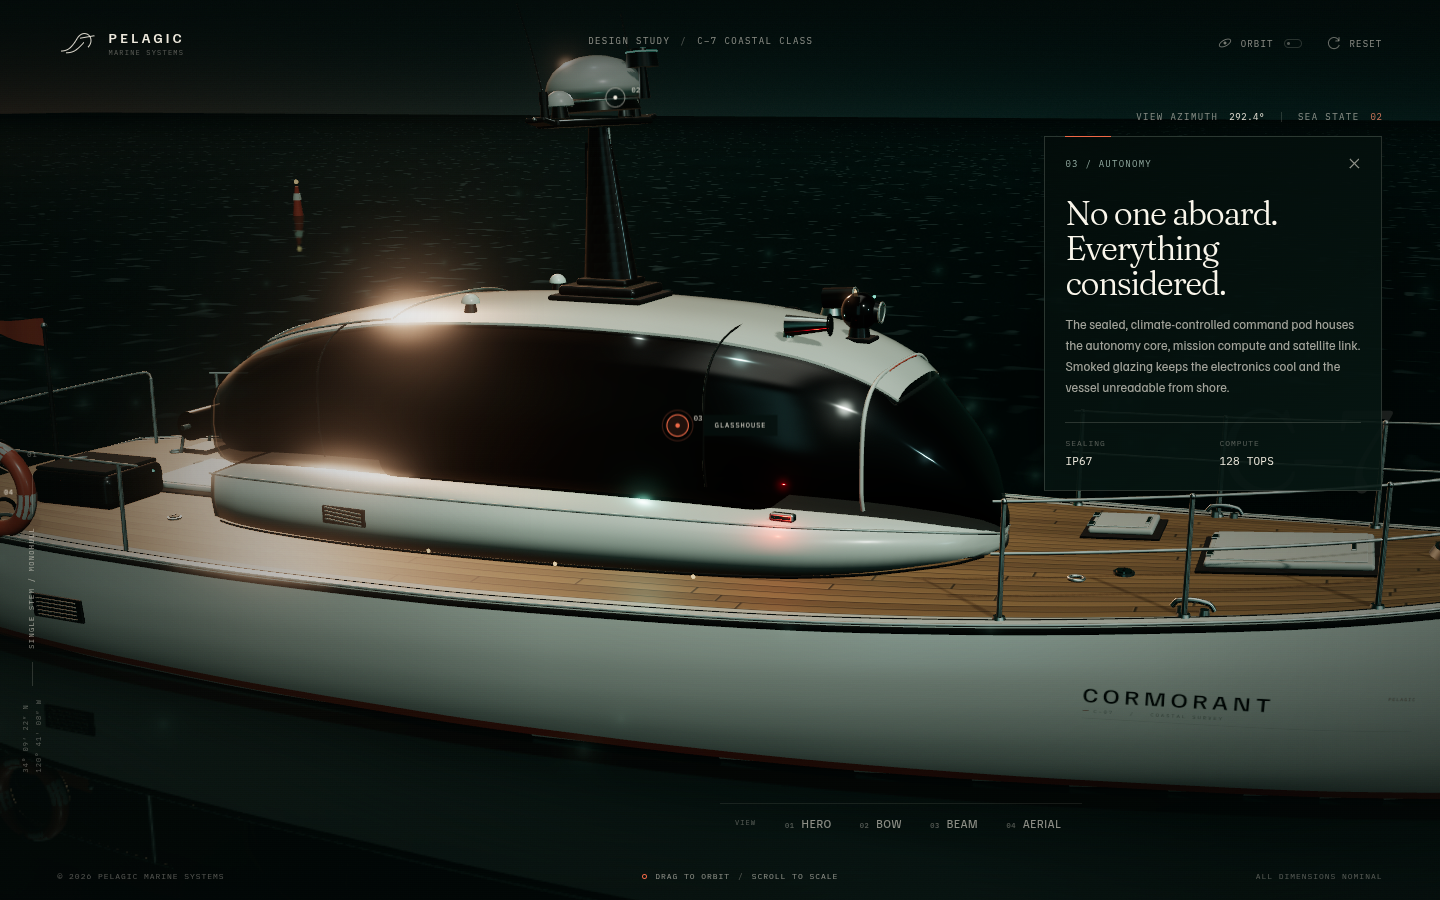
\includegraphics[width=\linewidth,height=0.31\textheight,keepaspectratio]{figures/detail.png}
\caption{局部视角：玻璃舱、硬顶、太阳能板、甲板边缘与传感器桅杆。}
\end{figure}

\begin{figure}[H]
\centering
\begin{minipage}[t]{0.30\linewidth}
  \centering
  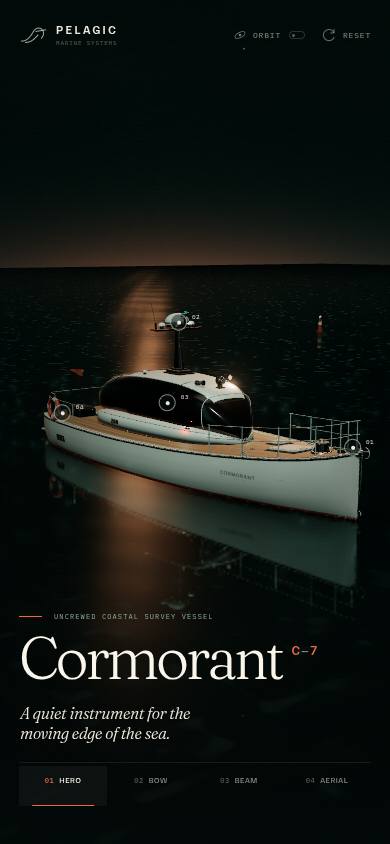
\includegraphics[height=0.27\textheight,keepaspectratio]{figures/mobile.png}
\end{minipage}\hfill
\begin{minipage}[t]{0.30\linewidth}
  \centering
  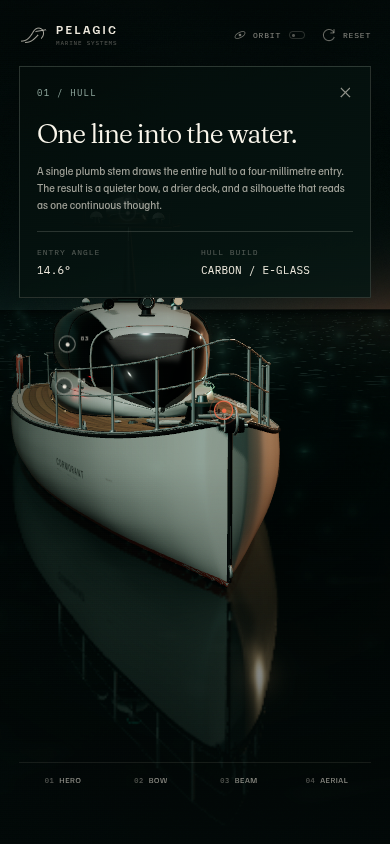
\includegraphics[height=0.27\textheight,keepaspectratio]{figures/mobile-detail.png}
\end{minipage}\hfill
\begin{minipage}[t]{0.34\linewidth}
  \vspace{0.25cm}
  {\small\color{sea}\textbf{移动端}}\\[0.18cm]
  {\footnotesize\color{stone}窄屏下使用更宽的视场和更远的相机；热点打开后，主标题退场，模型与结构说明占据画面。}
\end{minipage}
\caption{390\,px 移动端的两个观察状态。}
\end{figure}

\clearpage
\section{空 / SKYPRO XT}

同一个建模流程换到空中，得到的是 \texttt{drone/} 目录中的 SKYPRO XT 四轴航拍无人机：硬边机身、镜像三叶桨、三轴云台、实体起落架，以及程序化碳纤维、拉丝铝、镀膜镜片与夜航灯。亮色摄影棚与夜航模式共用一套结构，而不是两张互不相干的图。

\begin{figure}[H]
\centering
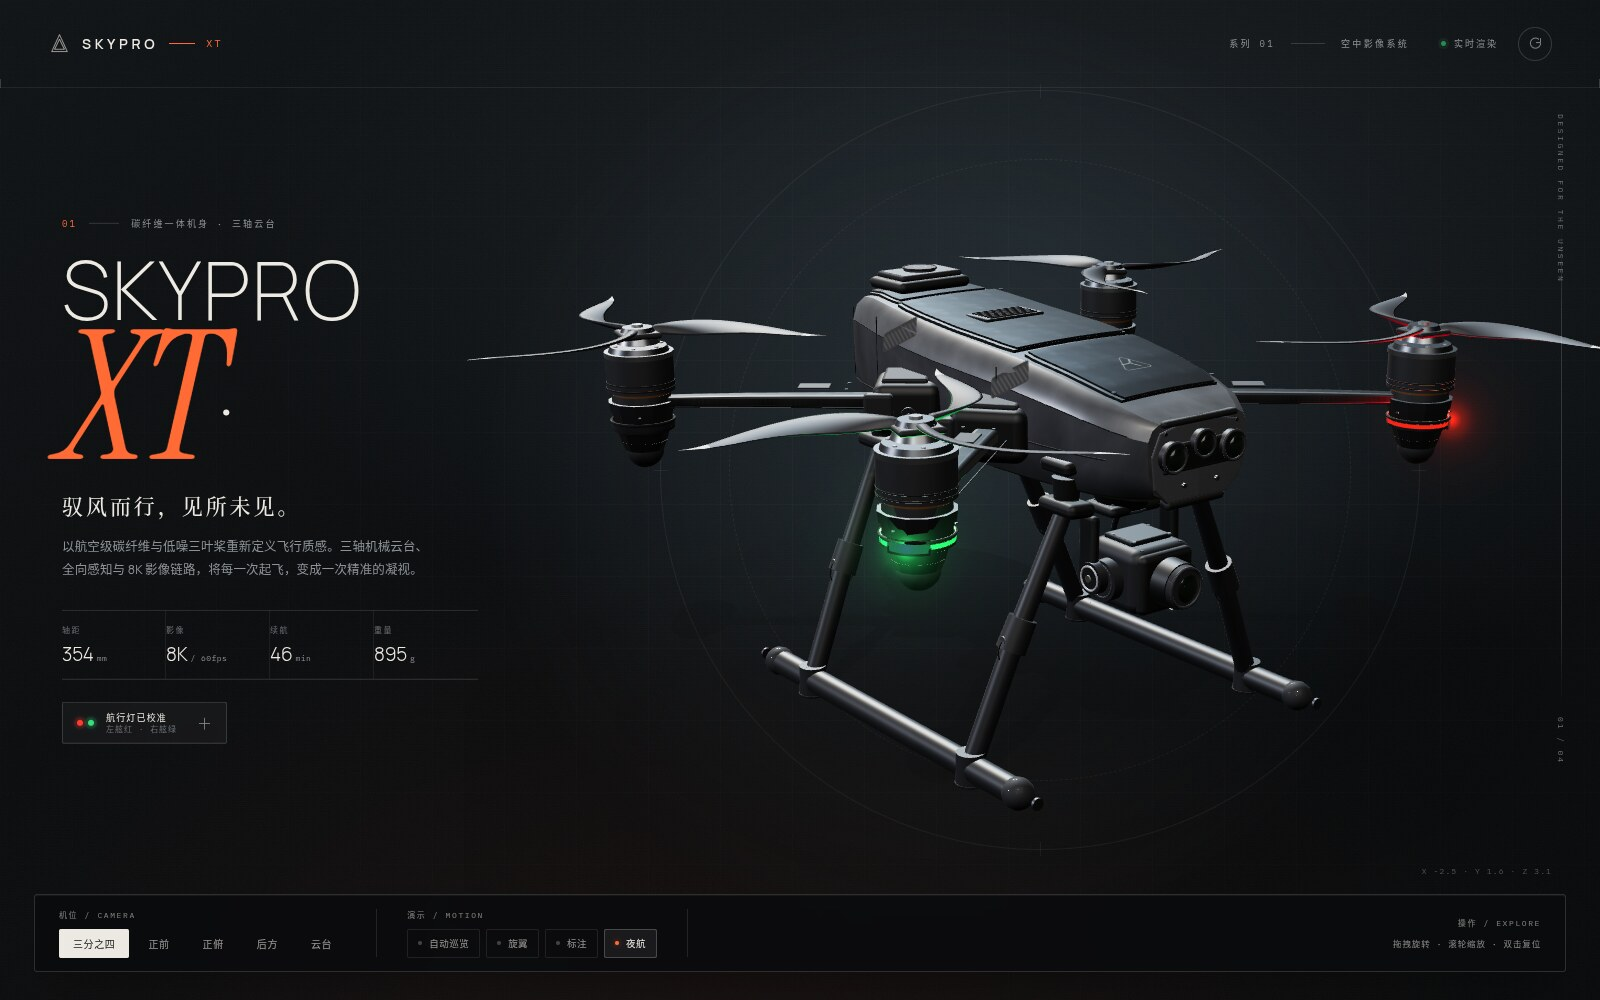
\includegraphics[width=\linewidth,height=0.30\textheight,keepaspectratio]{figures/drone-night.jpg}
\caption{SKYPRO XT 夜航模式：四轴、三轴云台与红绿航行灯。源码与截图位于本仓库 \texttt{drone/} 目录。}
\end{figure}

\begin{figure}[H]
\centering
\begin{minipage}[t]{0.55\linewidth}
  \centering
  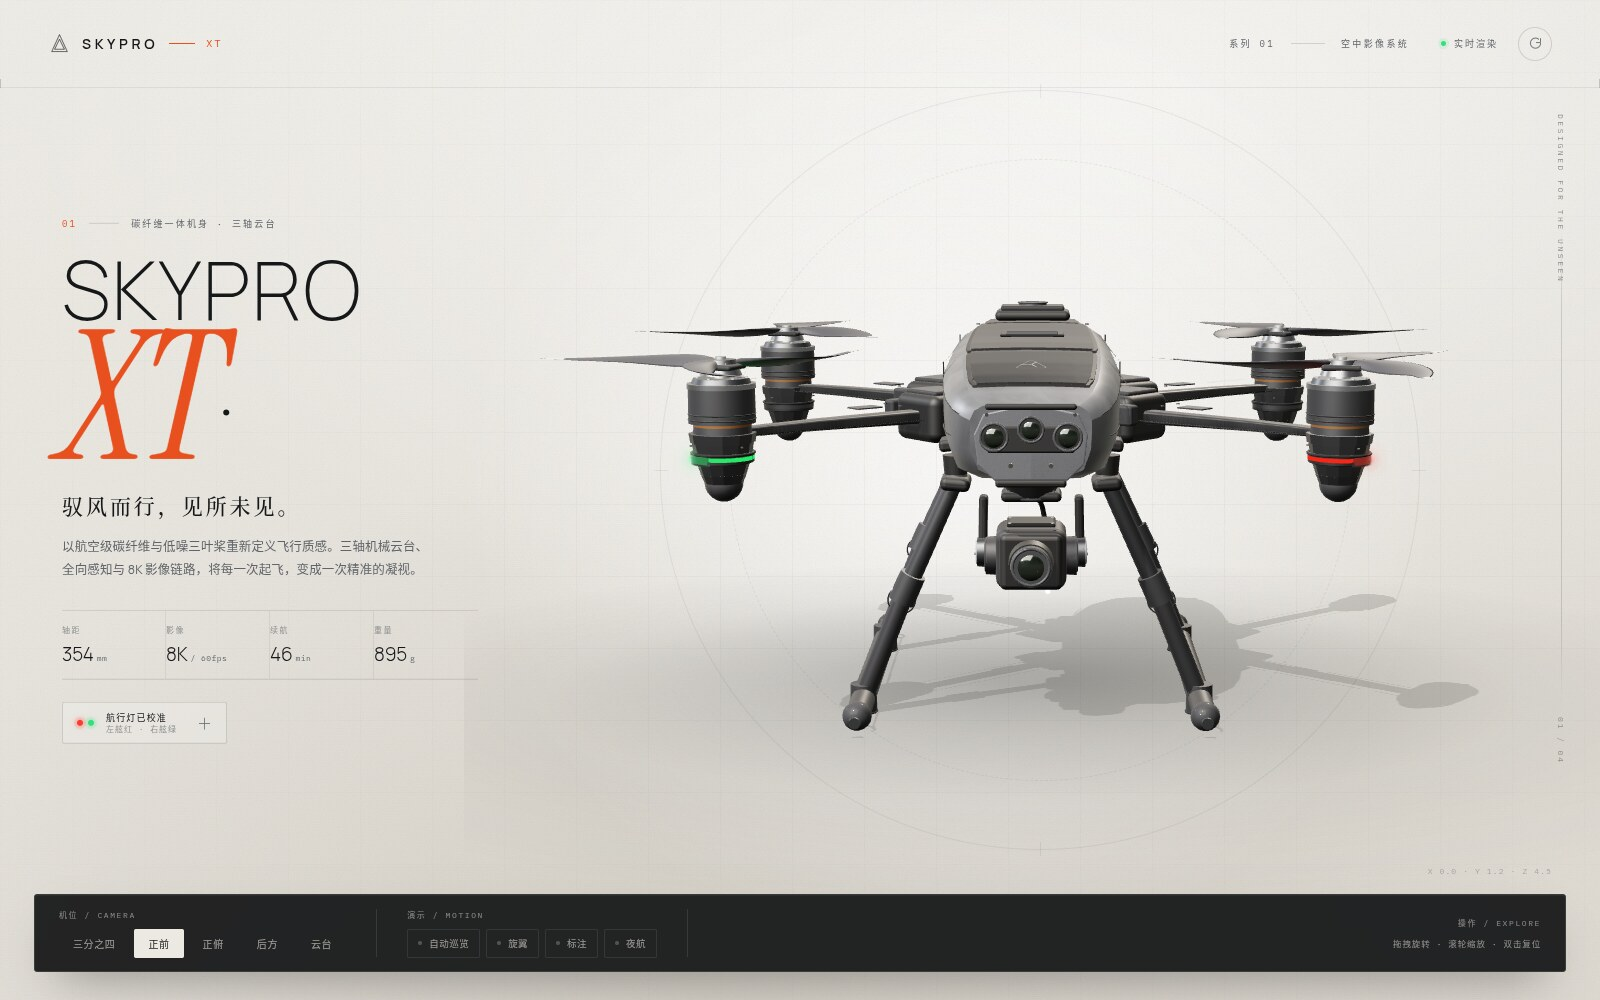
\includegraphics[width=\linewidth,height=0.21\textheight,keepaspectratio]{figures/drone-front.jpg}
\end{minipage}\hfill
\begin{minipage}[t]{0.40\linewidth}
  \centering
  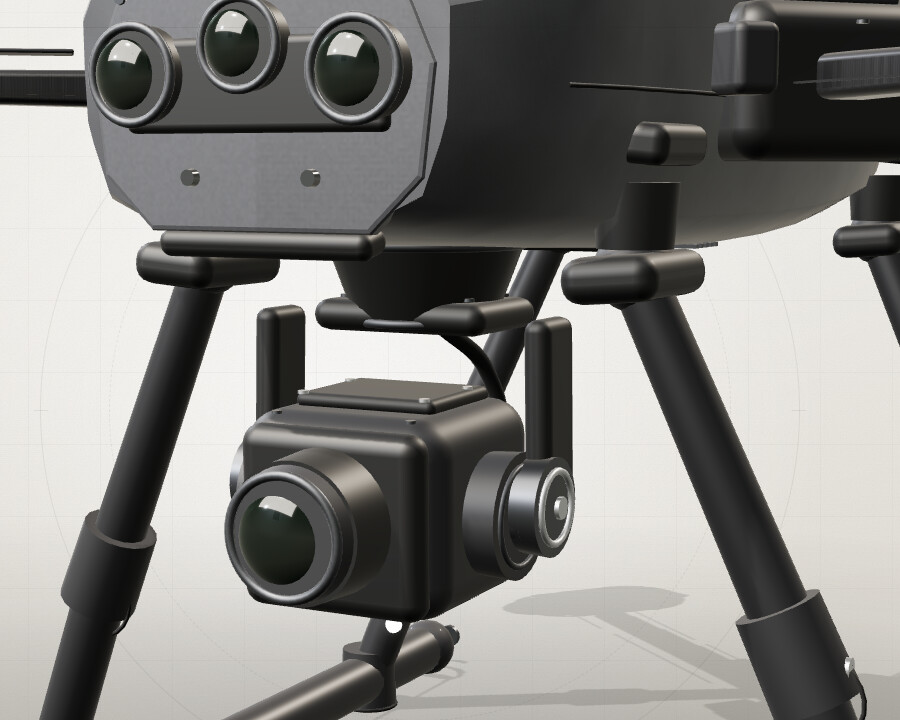
\includegraphics[width=\linewidth,height=0.21\textheight,keepaspectratio]{figures/drone-gimbal.jpg}
\end{minipage}
\caption{正前视角与云台实体挂载细节。}
\end{figure}

\vspace{0.2cm}
{\small\color{stone}
船与机共享的不是某个零件，而是从结构拆解、材质、光照到相机叙事的组织能力。完整交互与更多截图见仓库。\par}

\vspace{0.35cm}
{\small\color{seamist}仓库}\hspace{0.4em}
{\small\href{\repo}{\texttt{\repopath}}}\par
\vspace{0.08cm}
{\small\color{seamist}运行}\hspace{0.4em}
{\small\texttt{npm install \&\& npm run dev}}\par

\end{document}
